% Preámbulo
\documentclass[stu, 12pt, letterpaper, donotrepeattitle, floatsintext, natbib]{apa7}
\usepackage[utf8]{inputenc}
\usepackage{comment}
\usepackage{marvosym}
\usepackage{graphicx}
\usepackage{float}
\usepackage{amsmath}
\usepackage[normalem]{ulem}
\usepackage[spanish]{babel} 
\usepackage{indentfirst} %para le formato que quiere la profe QUITAR SI QUIERES OG APA7
\usepackage{ragged2e} %para le formato que quiere la profe QUITAR SI QUIERES OG APA7
\usepackage{indentfirst} %para le formato que quiere la profe QUITAR SI QUIERES OG APA7

\selectlanguage{spanish}
\useunder{\uline}{\ul}{}
\newcommand{\myparagraph}[1]{\paragraph{#1}\mbox{}\\}

% Portada
%\thispagestyle{empty}
\title{\Large Tarea 2 Unidad 5: Aspectos Matemáticos de las Principales Técnicas de Animación 2D}
\author{Abraham Jhared Flores Azcona} % (autores separados, consultar al docente)
% Manera oficial de colocar los autores:
%\author{Autor(a) I, Autor(a) II, Autor(a) III, Autor(a) X}
\affiliation{Instituto Tecnológico de Tijuana}
\course{SCC-1010SC5C: Graficación}
\professor{Dra. Martha Elena Pulido}
\duedate{8 de noviembre de 2021}

\begin{document}
    % Índices
    \pagenumbering{arabic}
    \maketitle

    % Cuerpo 
    %NOTA: PARA CITAR ESTILO "Merts (2003)" usar \cite{<nombre_cita_bib>}
    %    
    \newpage
    \section{Tweening}
    Estrictamente \begin{justifying}
      hablando, esta técnica recibe su nombre de la palabra ``between''. El nombre recae
      de la animación tradicional, donde el trabajo es dividido entre cuadros clave  y cuadros tween. \citep{penner-no-date} %citar a este dumbass:
      Se puede definir como una interpolación desde una posición hasta la otra, que puede expresarse como una función de tiempo:\par
    \end{justifying}
      \[p(t)=mt+b\]
    Donde \begin{justifying}
      \(m\) es la velocidad de cambio (pendiente), \(t\) es el tiempo y \(b\) es la posición inicial.\par
    \end{justifying}
    \vspace{\baselineskip}
    \section{Morphing}
    Es un \begin{justifying}
      efecto especial de la animación por computadora que consiste en moldea una imágen fotográfica de un objeto real a la imágen
      de otro objeto real. Entre ámbas imágenes se establecen puntos comunes generando digitalmente las etapas de transformación. \citep{prince-2015} %citar a NASA:
      \par
    \end{justifying}
    Estrictamente \begin{justifying}
      hablando, se usan los warps que (en este caso se utilizan vertices de triángulos) donde \(\textbf{V}_{\Delta}=c_1V_1+c_2V_2+c_3V_3\) y \(\textbf{W}_{\Delta}=c_1W_1+c_2W_2+c_3W_3\) y \(c_1+c_2+c_3=1\).
      Finalmente, lo que se hace es un mapeo de \(\textbf{V}\) hasta \(\textbf{A}\):
      \[\text{Morphing}= f:\textbf{V}\rightarrow\textbf{W}\]
    \end{justifying}
    \vspace{\baselineskip}
    \section{Onion y Skinning}
    Muy \begin{justifying}
      característico de los programas de animación e inclusive de la animación tradicional manual. Consiste en tener un ``fantasma'' del cuadro anterior
      al momento de dibujar ó creamos la siguiente; permite realizar animaciones con mayor fluidéz al saber en qué posición y forma se encontraba el cuadro anterior.\citep{unknown-author-2017}\par %citar a este:
    \end{justifying}
    \begin{figure}[H]
      \centering
      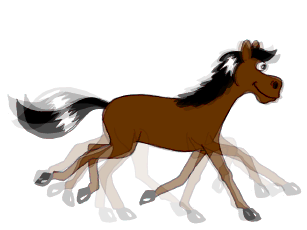
\includegraphics[width=8cm,height=6cm]{Onion_skin.png}
    \end{figure}
    \vspace{\baselineskip}
    \section{Interpolated rotoscoping}
    Es \begin{justifying}
      una técnica de animación que consiste en calcar o trazar directamente sobre una imágen en vivo. Se anima cuadro por cuadro el cortometraje
      consiguiendo una animación mucho más realista. \citep{ana-2021}%citar:
      \par
    \end{justifying}
    \begin{figure}[H]
      \centering
      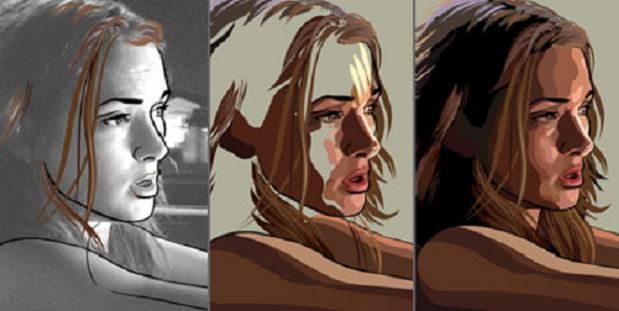
\includegraphics[width=10cm,height=6cm]{Rotoscoping-1.jpg}
    \end{figure}
    \vspace{\baselineskip}
    \newpage   
    % Referencias
    \renewcommand\refname{\textbf{Referencias}}
    \bibliography{referencias}
    
\end{document}